\documentclass[ngerman]{beamer}
\usetheme{metropolis}

% use \cref instead of autoref, autoref does not work with beamer
\usepackage{cleveref}

\usepackage{appendixnumberbeamer}


% some imports from handout, probably dont need all but whatever
\usepackage[utf8]{inputenc}
\usepackage[T1]{fontenc}   
\usepackage{graphicx}       
\usepackage[german]{babel}
\usepackage{csquotes}     
\usepackage{eurosym}
\usepackage{float}
\usepackage{rotating}
\usepackage{blkarray}
\usepackage{amsmath}
\usepackage{amssymb}
\usepackage{gensymb}
\usepackage{amsthm}
\usepackage{listings}
\usepackage{caption}
\usepackage{subcaption}
\usepackage{interval}
\usepackage{textpos}
\usepackage[style=authoryear, backend=biber]{biblatex}
\addbibresource{references.bib}


% argmin command
\newcommand{\argmin}[1]{\underset{#1}{\operatorname{arg}\,\operatorname{min}}\;}
% command for euclidean norm
\newcommand{\norm}[1]{\lVert#1\rVert}
% command for lagrangian L (kind of handwritten L)
\newcommand{\Lagr}{\mathcal{L}}

% show current page number in footer
\setbeamertemplate{footline}[frame number]


% No navigation symbols at the slides' bottom
\beamertemplatenavigationsymbolsempty

% command for creating a frame with one full-slide image without caption
% first arg: frame title, second arg: path to img
\newcommand {\imageframe}[2] {
	\begin{frame}{#1}
		\begin{center}
			\begin{figure}
			\includegraphics[width=\textwidth,height=0.8\textheight,keepaspectratio]{#2}
		\end{figure}
		\end{center}
	\end{frame}
}



\title{Support Vector Machines}
\author{André Hopfgartner \& Matthias Rupp}
\institute{Vorarlberg University of Applied Sciences \\ \\ \\ \\ \\ \\ 
\includegraphics[width=0.35\textwidth]{assets/Logo-A3.png}}

\date{08.06.2021}

\begin{document}

\begin{frame}[plain]
    \maketitle
\end{frame}


\begin{frame}{Agenda}
	\setbeamertemplate{section in toc}[sections numbered]
	\tableofcontents[hideallsubsections]
\end{frame}


\section{Einführung}


\begin{frame}{Intuition}
	\emph{Ziel}: lineare Trennung zweier Klassen\\ \pause
	\emph{Wie?}: Definition einer (Hyper-) Ebene \\ \pause
	\emph{Nebenbedingung}: Möglichst großer freier Bereich\\ \pause
	
	\begin{center}
		\begin{figure}
			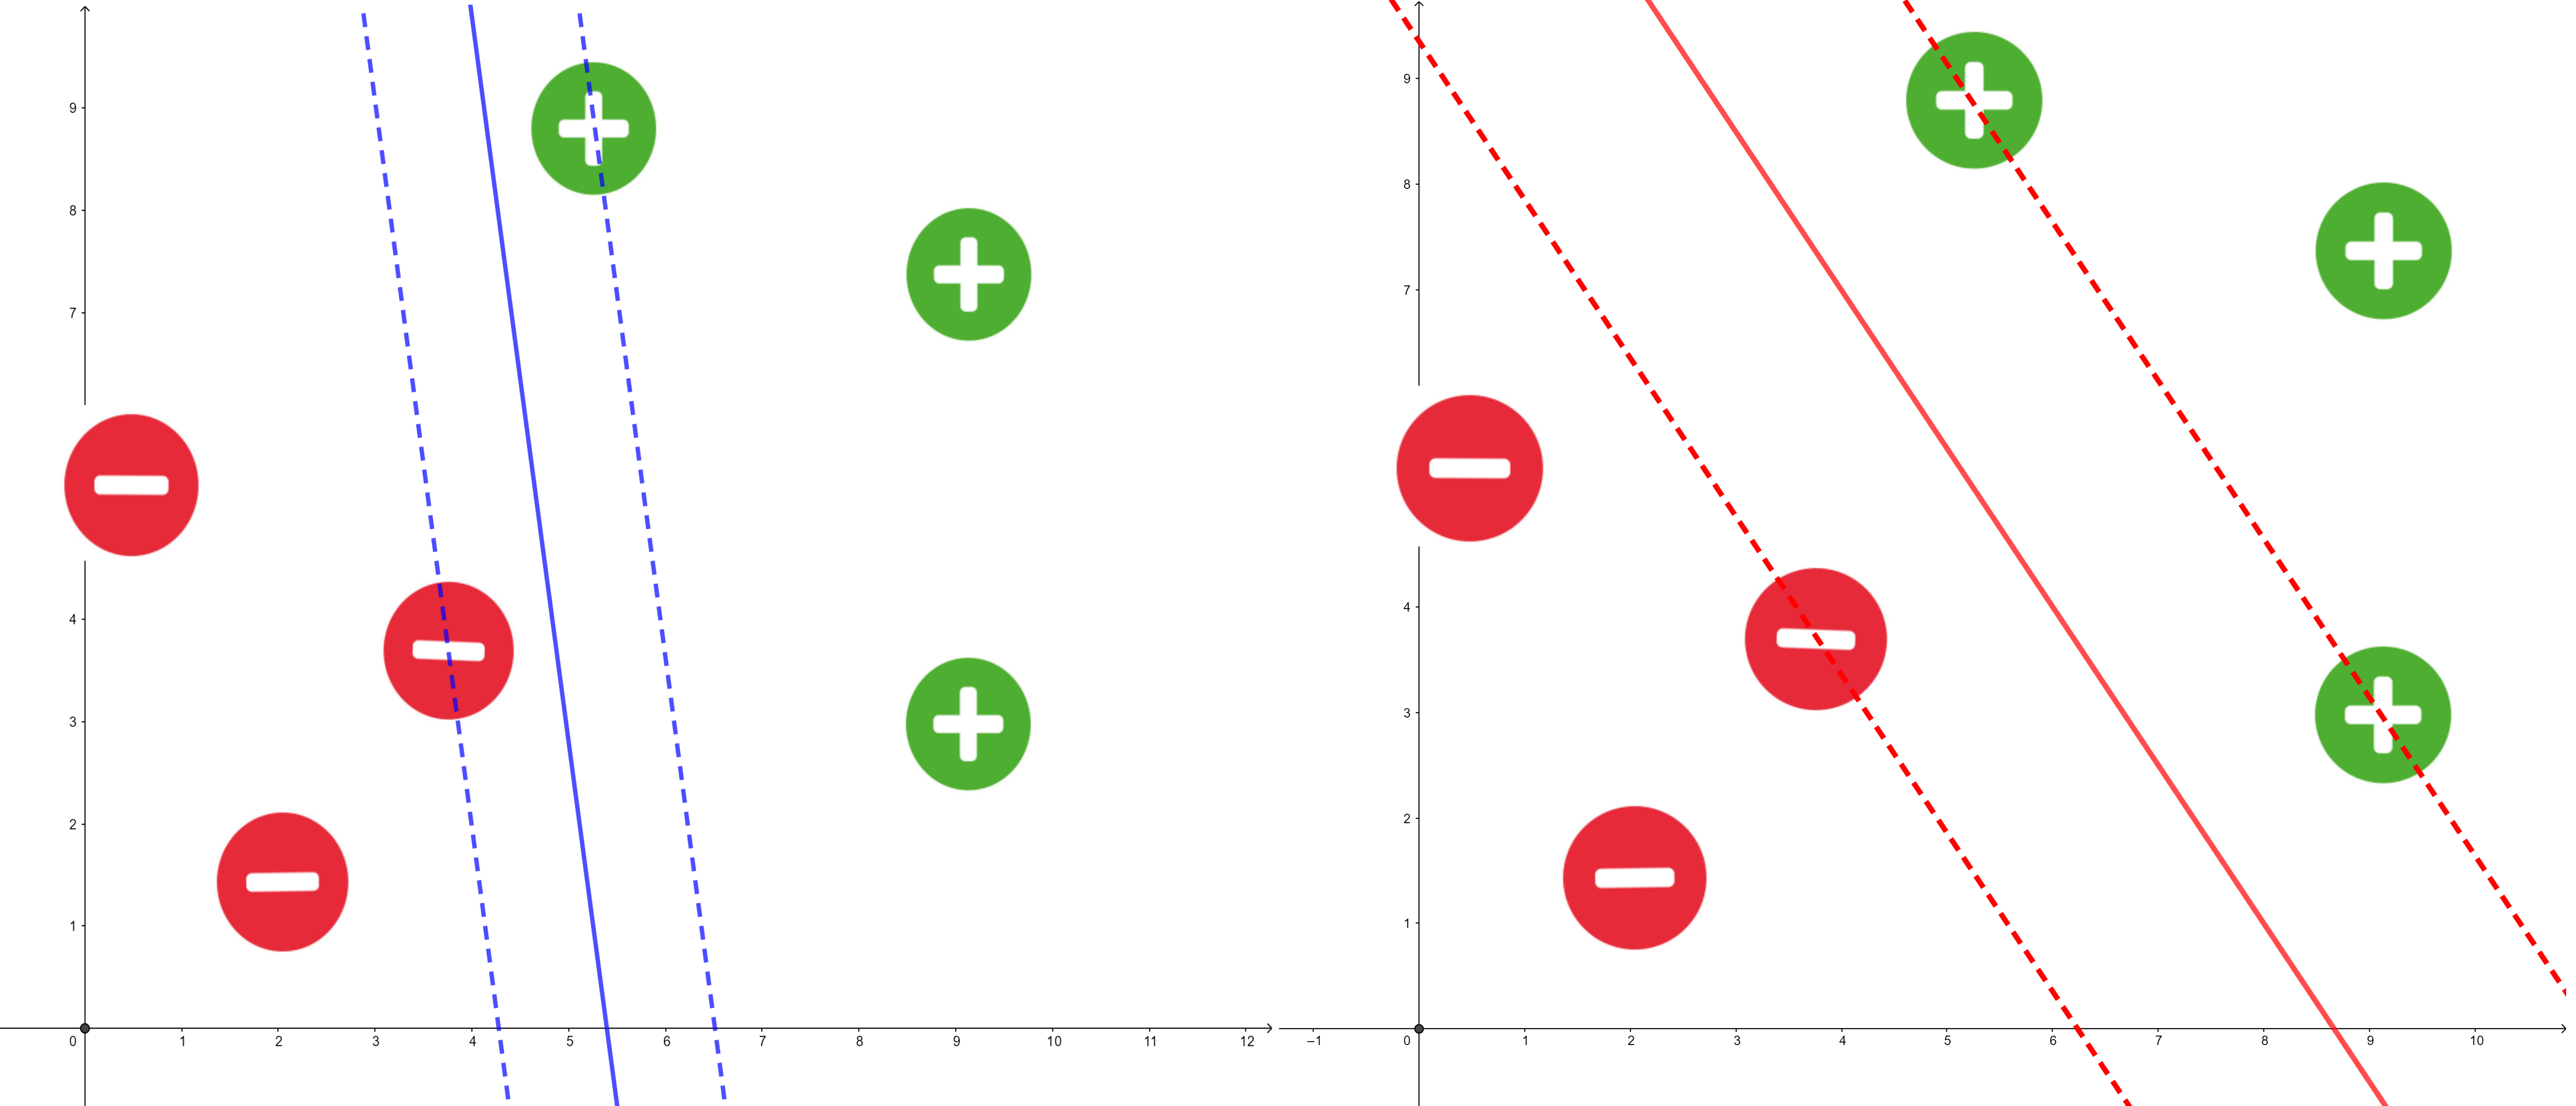
\includegraphics[width=\textwidth,height=0.7\textheight,keepaspectratio]{assets/small_vs_big_margin.png}
		\end{figure}
	\end{center}	
\end{frame}

\begin{frame}{Arten von SVM}
	\emph{Arten von SVM:}
	\begin{itemize}
		\item \emph{Hard-Margin SVM}: Daten werden 100\% korrekt getrennt
		\item \emph{Soft-Margin SVM}: Einzelne Datenpunkte können falsch klassifiziert werden um insgesamt bessere Trennung zu erhalten
	\end{itemize}

	\begin{center}
		\begin{figure}
			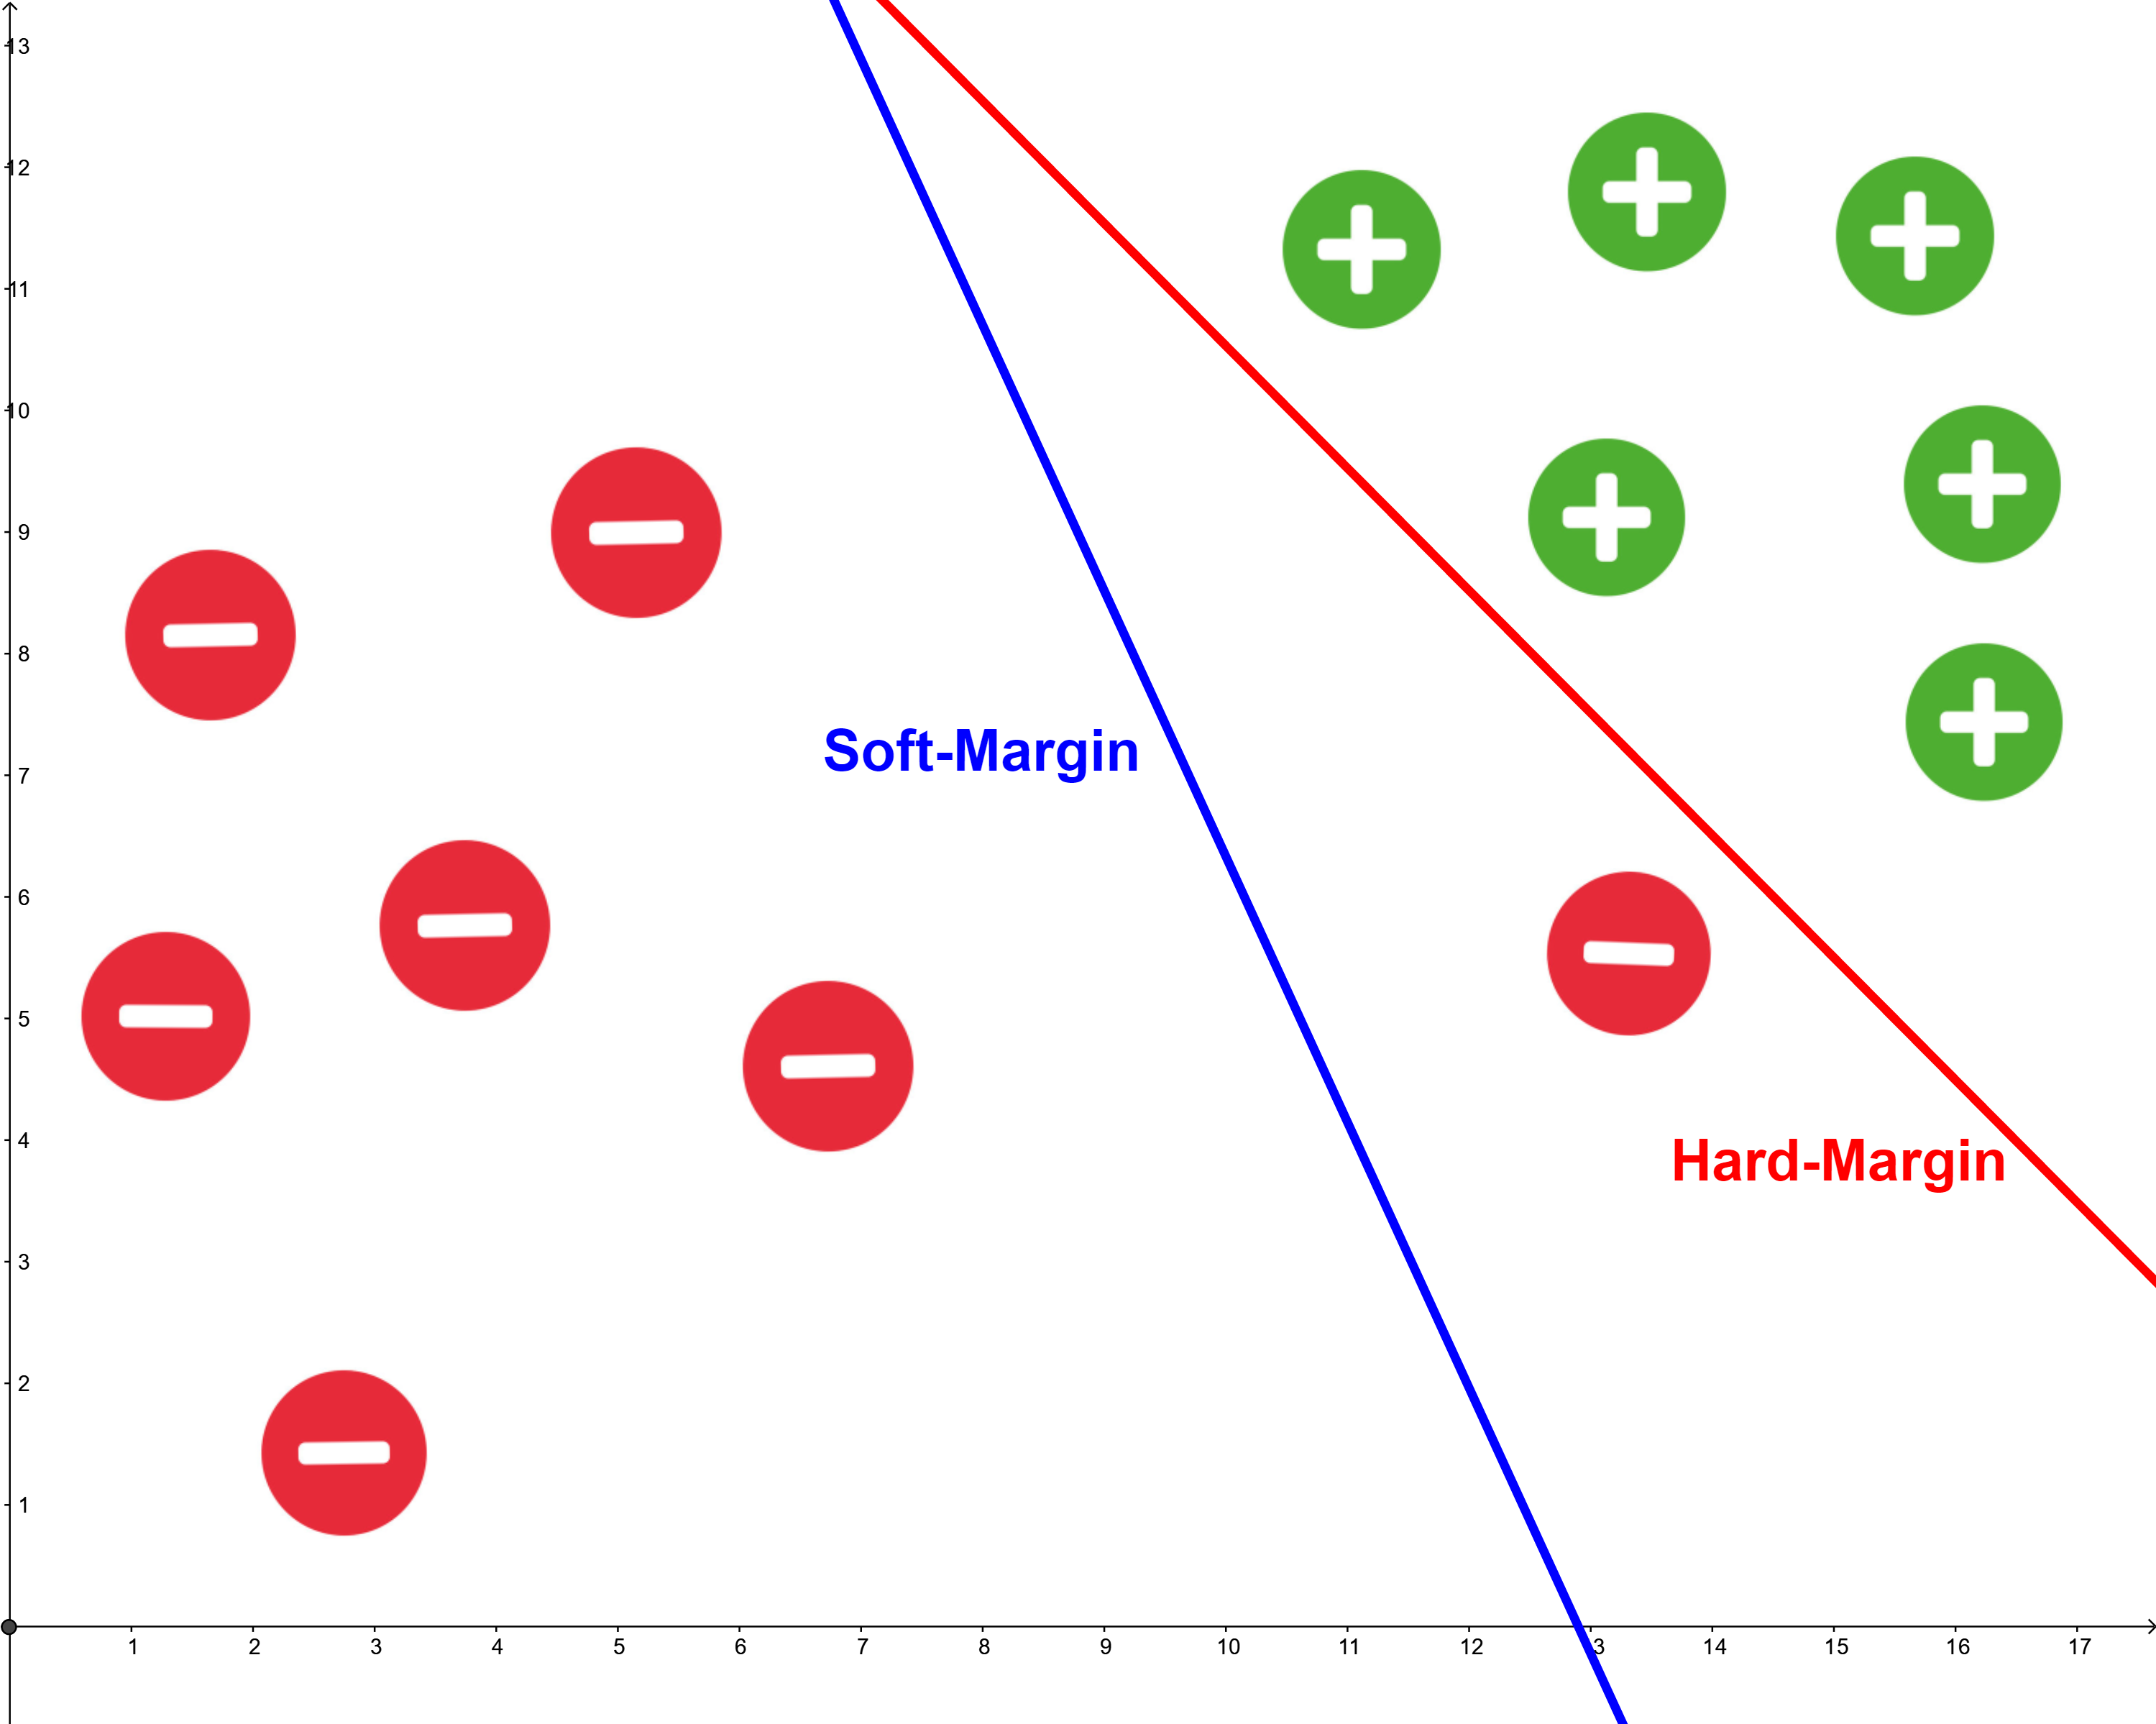
\includegraphics[width=\textwidth,height=0.6\textheight,keepaspectratio]{assets/hard_vs_soft_margin.png}
		\end{figure}
	\end{center}

\end{frame}

\section{Hard-Margin Support Vector Machine}


\begin{frame}{Mathematische Formulierung}
	
\end{frame}


\begin{frame}{Trennungsebene}
	
	Für die Trennungsebene gilt:
	\begin{equation} \label{plane_eq}
		\begin{aligned}
			w^{T} x_{n} + b &= 0 \\
		\end{aligned}
	\end{equation}
	\pause
	
	Klassifikation über Vorzeichen:
	\begin{subequations} \label{svm_classify1}
		\begin{alignat*}{2}
			y = sign(w^{T} x + b)  & \qquad & \text{ ist gleichbedeutend mit} \\
			w^{T} x + b > 0 & & \text{ für } y = +1\\
			w^{T} x + b < 0 & & \text{ für } y = -1
		\end{alignat*}
	\end{subequations}

\end{frame}



\begin{frame}{Soft-Margin SVM}
Formuliert als Optimierungsproblem:
	
\begin{subequations} \label{final_lagrange_soft}
	\begin{alignat*}{2}
		&\!\max_{\alpha}        &\qquad&  	\Lagr(\alpha) = \sum_{n=1}^{N} \alpha_{n} - \frac{1}{2} \sum_{n=1}^{N} \sum_{m=1}^{M} y_{n} y_{m} \alpha_{n} \alpha_{m} x_{n}^{T} x_{m} \\
		&\text{mit } &      & 0 \leq \alpha_{n} \leq C \text{ für } n=1..N \\
		&       & & \sum_{n=1}^{N} \alpha_{n} y_{n} = 0\text{ für } n=1..N
	\end{alignat*}
\end{subequations}

\end{frame}


\begin{frame} {A test with images}
	\framesubtitle{subcaption testing with images}
	\begin{minipage}{0.5\textwidth}

		\begin{itemize}
			\item Some 
			\item text 
			\item on left side of slide here..
			\item \cref{fig:intuition_margin} zeigt blabla.
		\end{itemize}
		\pause
	\end{minipage} \hfill
	\begin{minipage}{0.45\textwidth}
	\begin{figure}
		\centering
		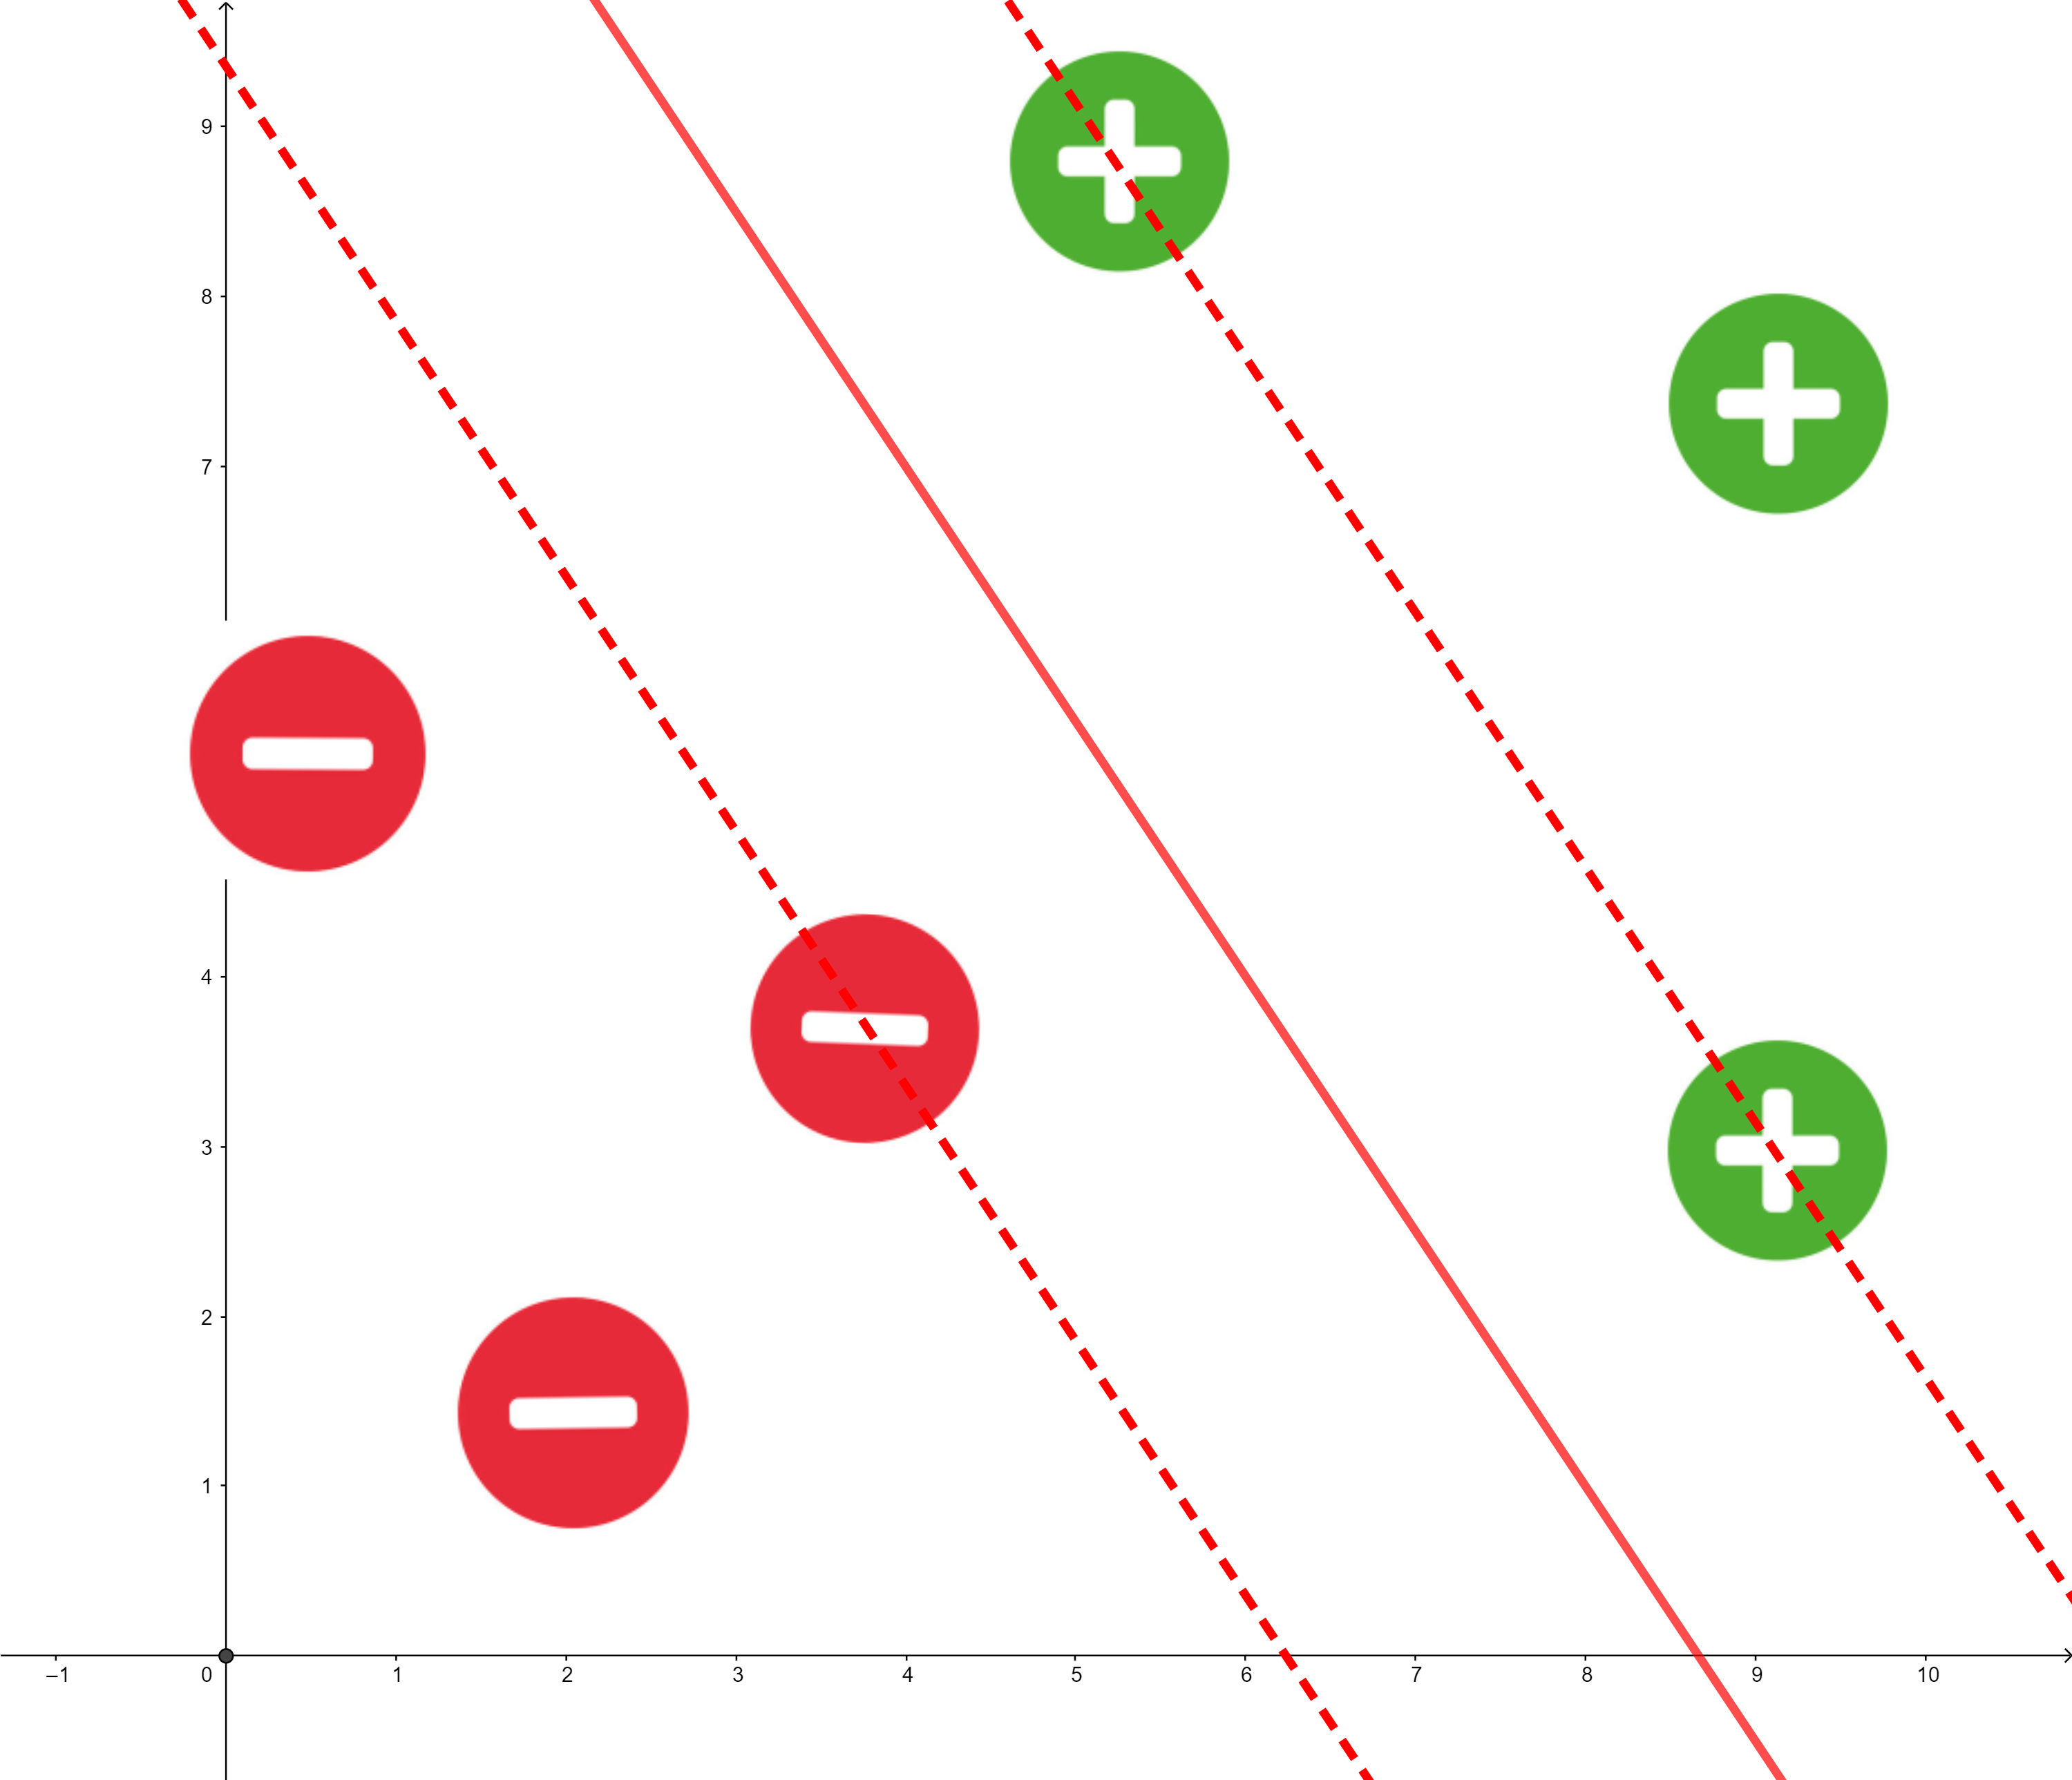
\includegraphics[height=0.9\textwidth]{assets/intuition_big_margin.png}
		\caption{Abhängig von der Lage der Trennebene entstehen schmale (blau) oder breite (rot) Trennbänder. Ziel ist die Maximierung der Breite des Trennbands durch die Ermittlung der optimalen Lage der Trennebene.}
		\label{fig:intuition_margin}
	\end{figure}
	\end{minipage}
\end{frame}

\begin{frame}
	\begin{subequations} \label{svm_classify1}
		\begin{alignat}{2}
			y = sign(w^{T} x + b)  & \qquad & \text{ gleichbedeutend mit} \\
			w^{T} x + b > 0 & & \text{ für } y = +1\\
			w^{T} x + b < 0 & & \text{ für } y = -1
		\end{alignat}
	\end{subequations}

	In \cref{svm_classify1} wird .. \\
	
	Footcite example \footcite{platt_sequential_1998} \\
	
	\textcite{burges_tutorial_1998}
\end{frame}


\section{Soft-Margin Support Vector Machine}

\section{Vergleich Hard- \& Soft-Margin Support Vector Machine}

\section{Nichtlineare Trennung}



\begin{frame}[standout]
	Fragen?
\end{frame}

\begin{frame}
	\printbibliography
\end{frame}



\end{document}



